%!TEX root = ../Pflichtenheft.tex

\chapter{Benutzeroberfläche}
\label{chap:ui}

\section{Haupseite und Buchung}

Die Startseite der Anwendung ist in \ref{fig:startseite} dargestellt.
Auf dieser haben NutzerInnen die Möglichkeit, dem Raum zu buchen oder auf andere Ansichten zu wechseln.
Der Banner in allen Ansichten zeigt den aktuellen Raumstatus an.
Insbesondere wird dadurch die Priorität der aktuellen Buchung mithilfe der Farbe des Banners angezeigt.

Rechts in dieser Ansicht befindet sich ein Kalender, der die aktuelle Woche und die Buchungen in diesem Zeitraum anzeigt.
Die Buchungen sind farblich nach Priorität gekennzeichnet, weitere Informationen können durch Klicken auf die Buchung eingesehen werden.
Neben dieser Möglichkeit, den Raum zu buchen, gibt es je nach Anmeldungsstatus einen Anmelde- oder Abmeldebutton und einen separaten Buchungsbutton für NutzerInnen,
für die die Verwendung des Kalenders Probleme bereitet.
Falls zur Zeit der Verwendung eine Buchung des Nutzenden stattfindet, wird ein Quick-Checkout Button angezeigt,
der es ermöglicht, den Raum schnell freizugeben.
\begin{figure}[ht]
    \centering
    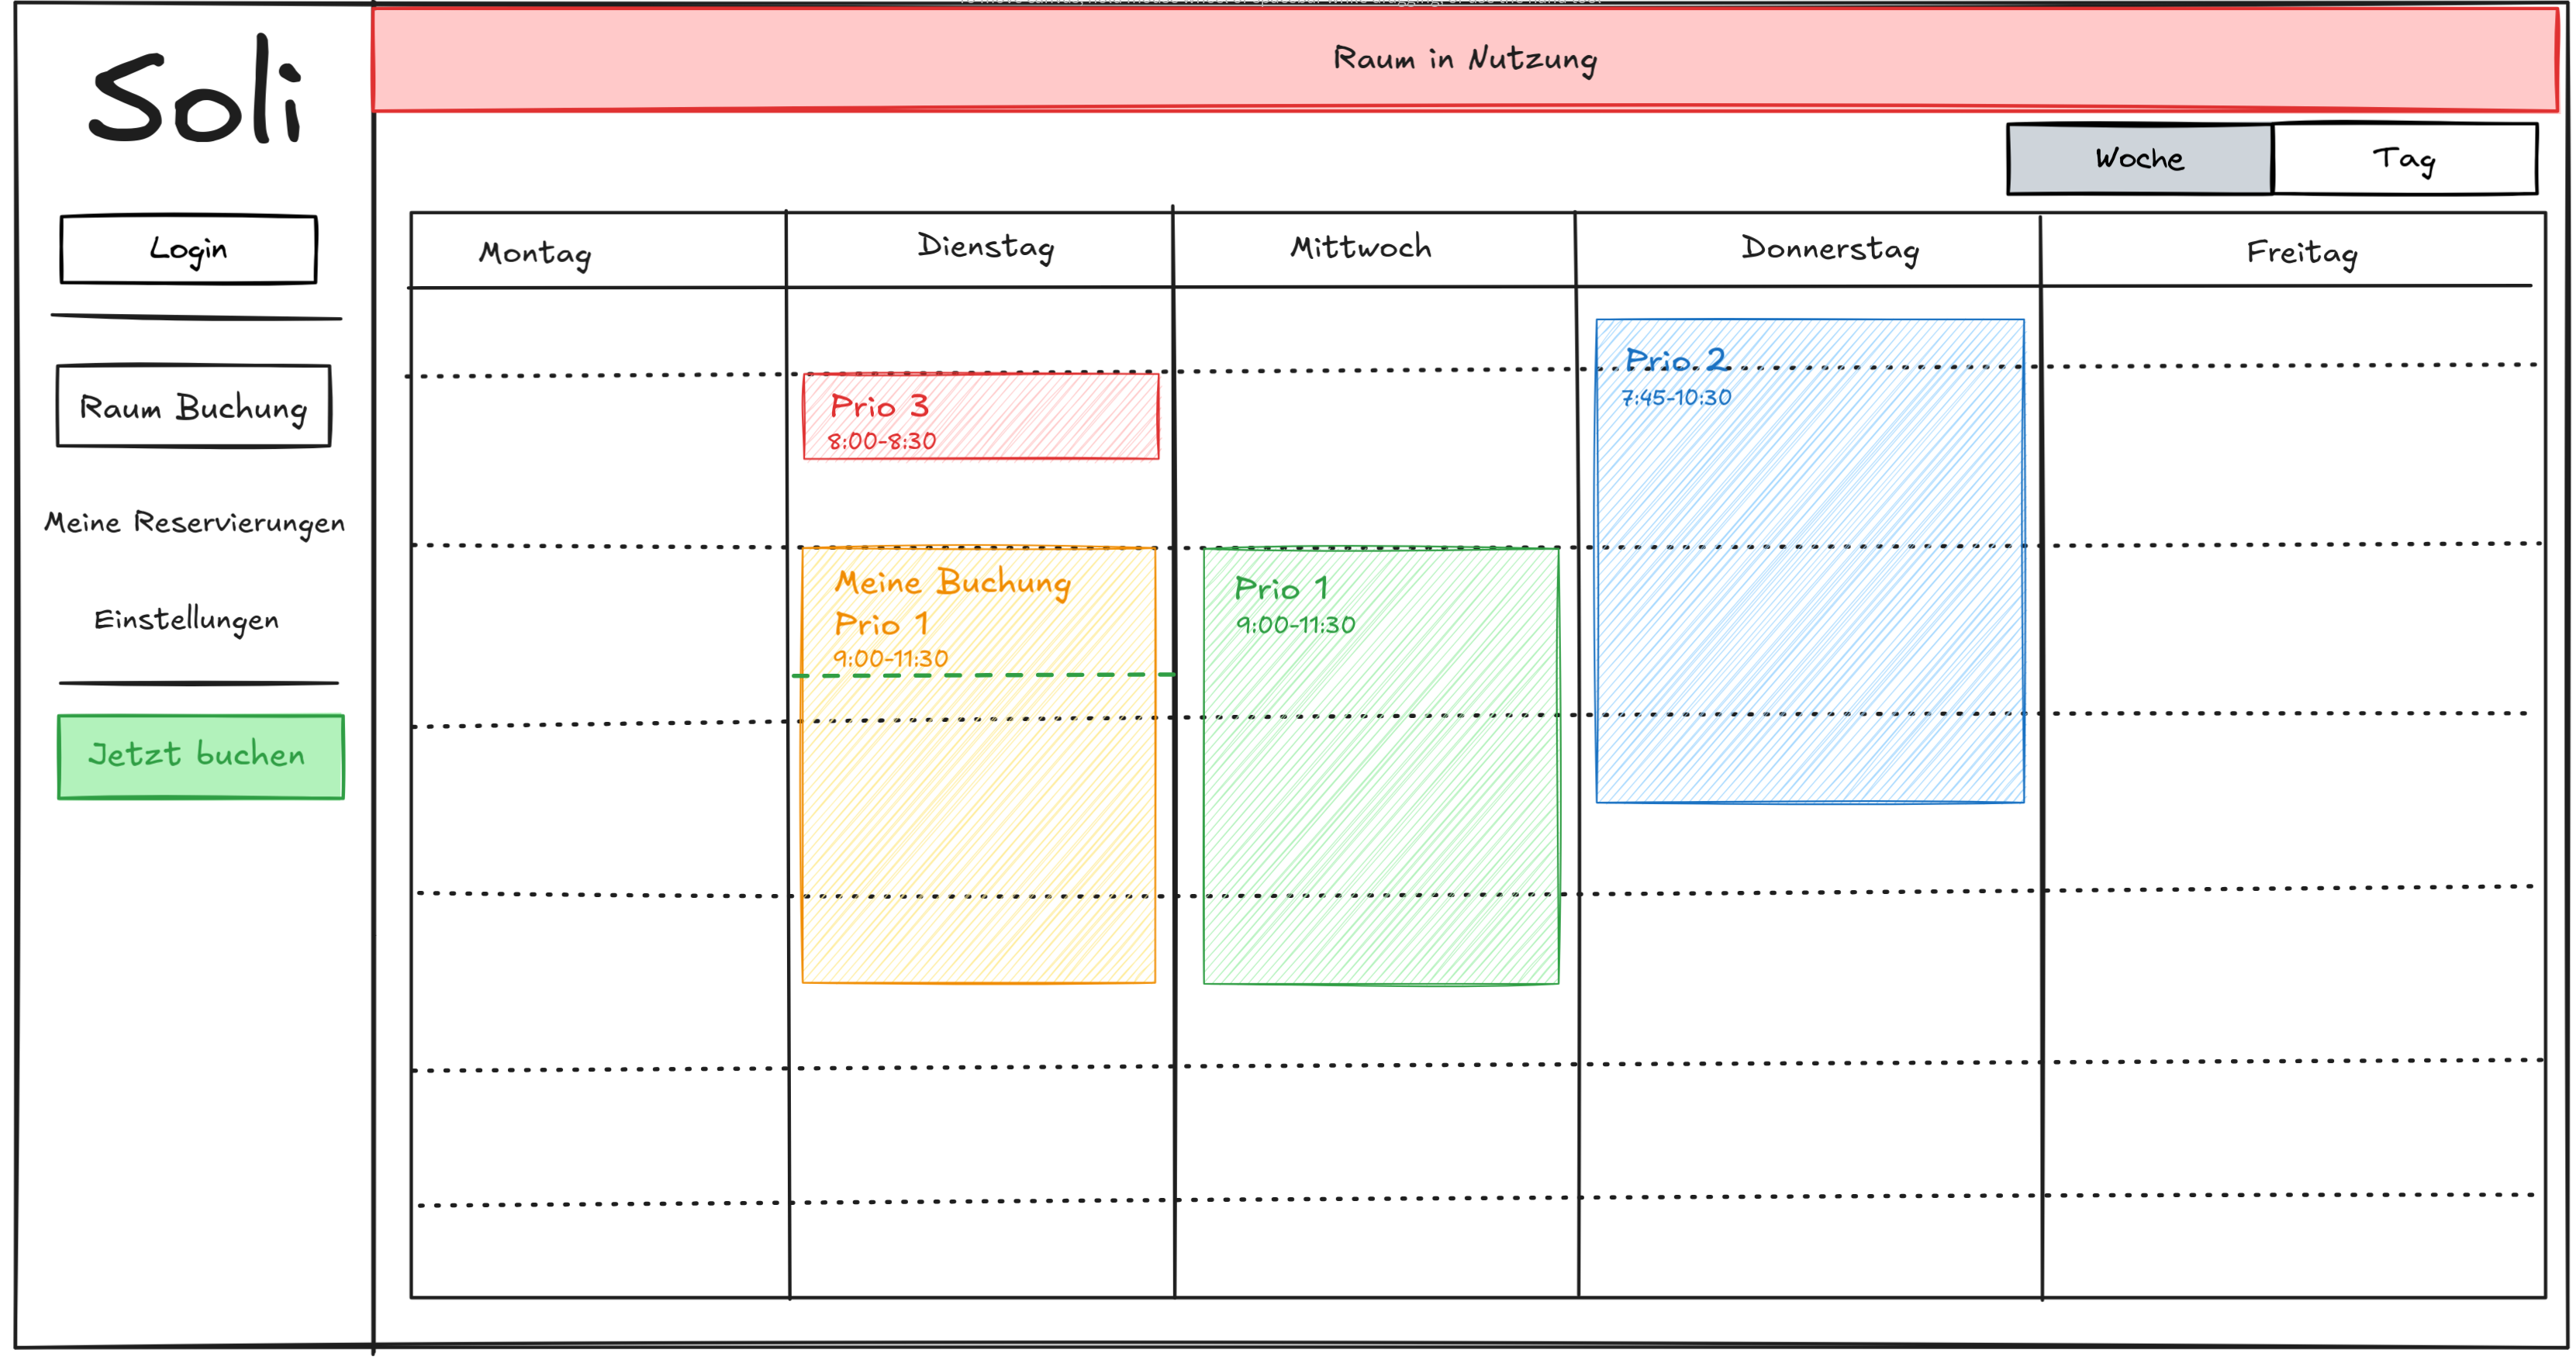
\includegraphics[scale=0.15]{figures/ui/startseite}
    \caption{Startseite der Anwendung}
    \label{fig:startseite}
\end{figure}
\clearpage

Sollten Nutzende eine Buchung vornehmen wollen, so klicken diese in den gewünschten Zeitraum
und es wird der Dialog in \ref{fig:buchung} dargestellt.

Der Dialog bietet Nutzenden die Möglichkeit, den genauen Start- und Endzeitpunkt der Buchung festzulegen.

Außerdem können Nutzende die Priorität der Buchung in Form einer Zahl zwischen 1 und 3 festlegen.
Nutzende können auch angeben, ob sie bereit sind, den Raum mit anderen Nutzenden zu teilen.
Für diesen Zweck werden ihnen drei Optionen bereitgestellt: "Ja", "Nein" und "Auf Anfrage".
Deren Bedeutung wird in \change{Wo definieren wir das?} genauer erläutert.

Letztlich können Nutzende eine Beschreibung für die Buchung hinterlegen, die anderen angemeldeten Nutzenden angezeigt wird.
\begin{figure}[ht]
    \centering
    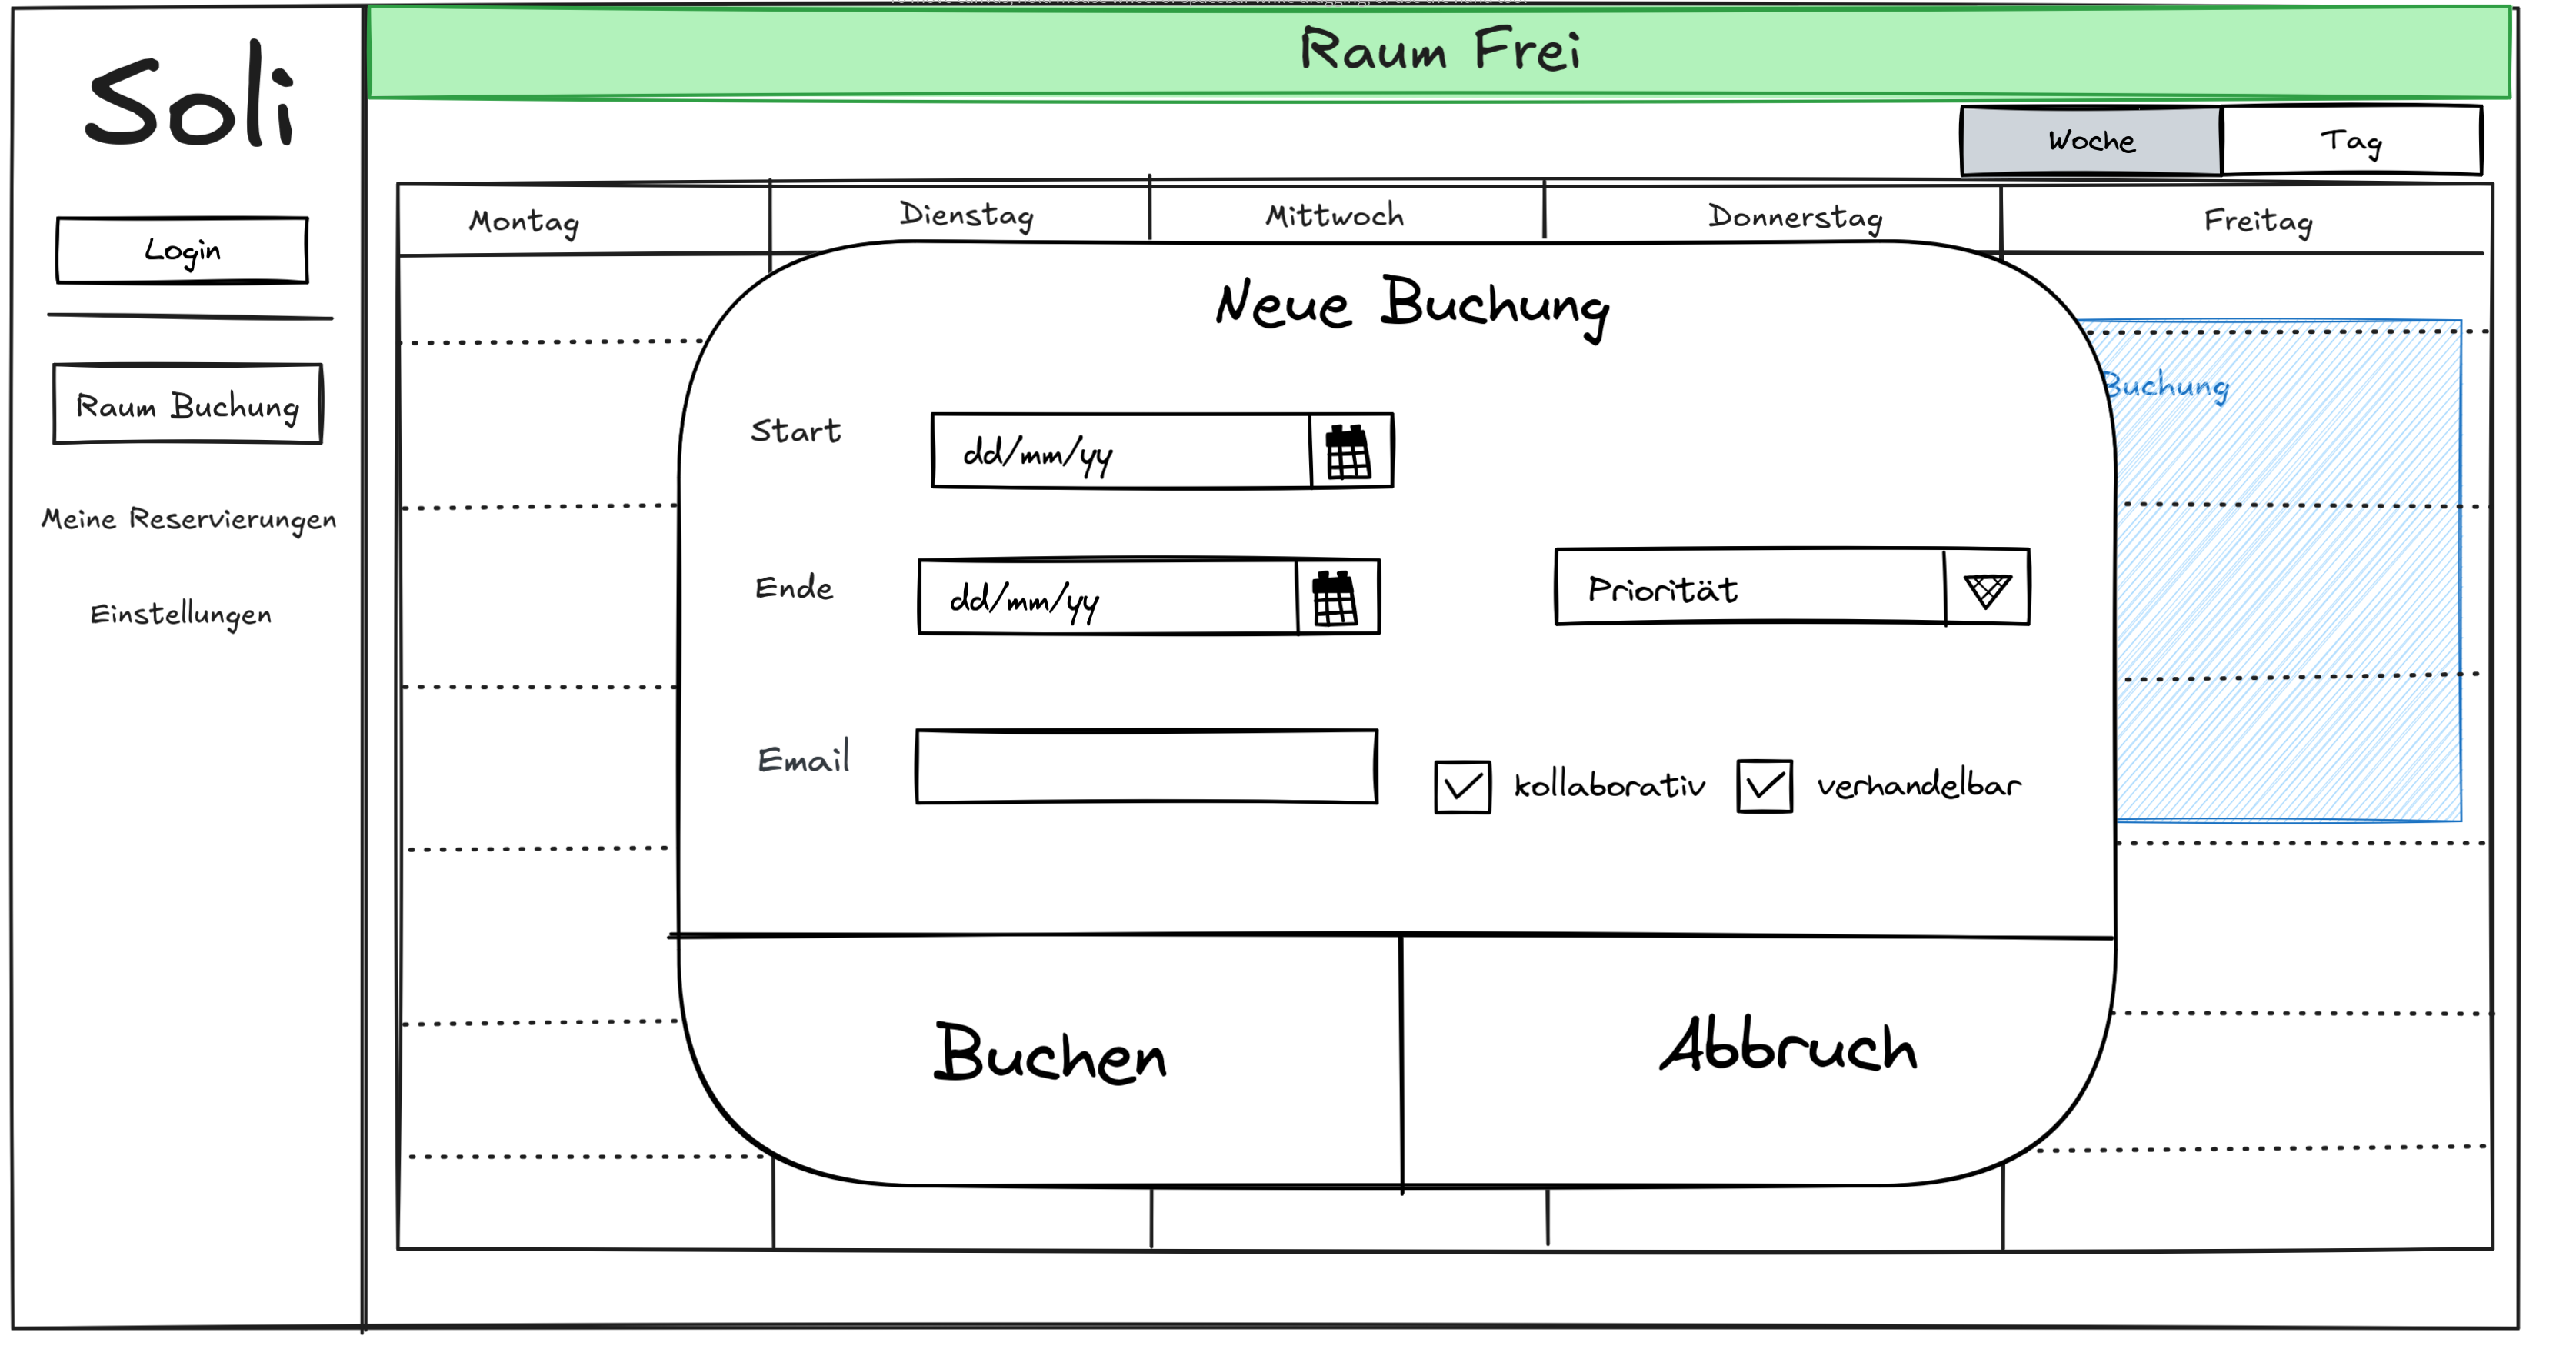
\includegraphics[scale=0.15]{figures/ui/buchungsdialog}
    \caption{Buchungsdialog}
    \label{fig:buchung}
\end{figure}
\clearpage

Tätigen Nutzende eine Buchung, so werden diese aufgefordert, sich anzumelden.
Der hierzu gehörige Dialog ist in \ref{fig:login} dargestellt.
Alternativ ist dieser Dialog auch über den Anmeldungsbutton, der in Abbildung \ref{fig:startseite} zu sehen ist, erreichbar.

In diesem Dialog wird Nutzenden die Möglichkeit gegeben, sich mit ihrem KIT-Konto, mit einem lokalen Gastkonto oder als Administrator anzumelden.

Falls Nutzende die Anmeldung per KIT-Konto wählen, werden sie auf die KIT-Login-Seite weitergeleitet.
Von dort aus können sie sich mit ihren KIT-Zugangsdaten anmelden.

Falls Nutzende die Anmeldung per Gastkonto wählen, werden sie aufgefordert, eine E-Mail-Adresse anzugeben.
Mit der Bestätigung dieser E-Mail-Adresse wird ein temporäres Gastkonto erstellt und die Anmeldung per Cookie gespeichert.

Falls Nutzende die Anmeldung als Administrator wählen, werden sie aufgefordert, den Nutzernamen und das Passwort des Administrators einzugeben.

Nach einer erfolgreichen Anmeldung werden Nutzende auf die nächste Seite weitergeleitet.
\begin{figure}[ht]
    \centering
    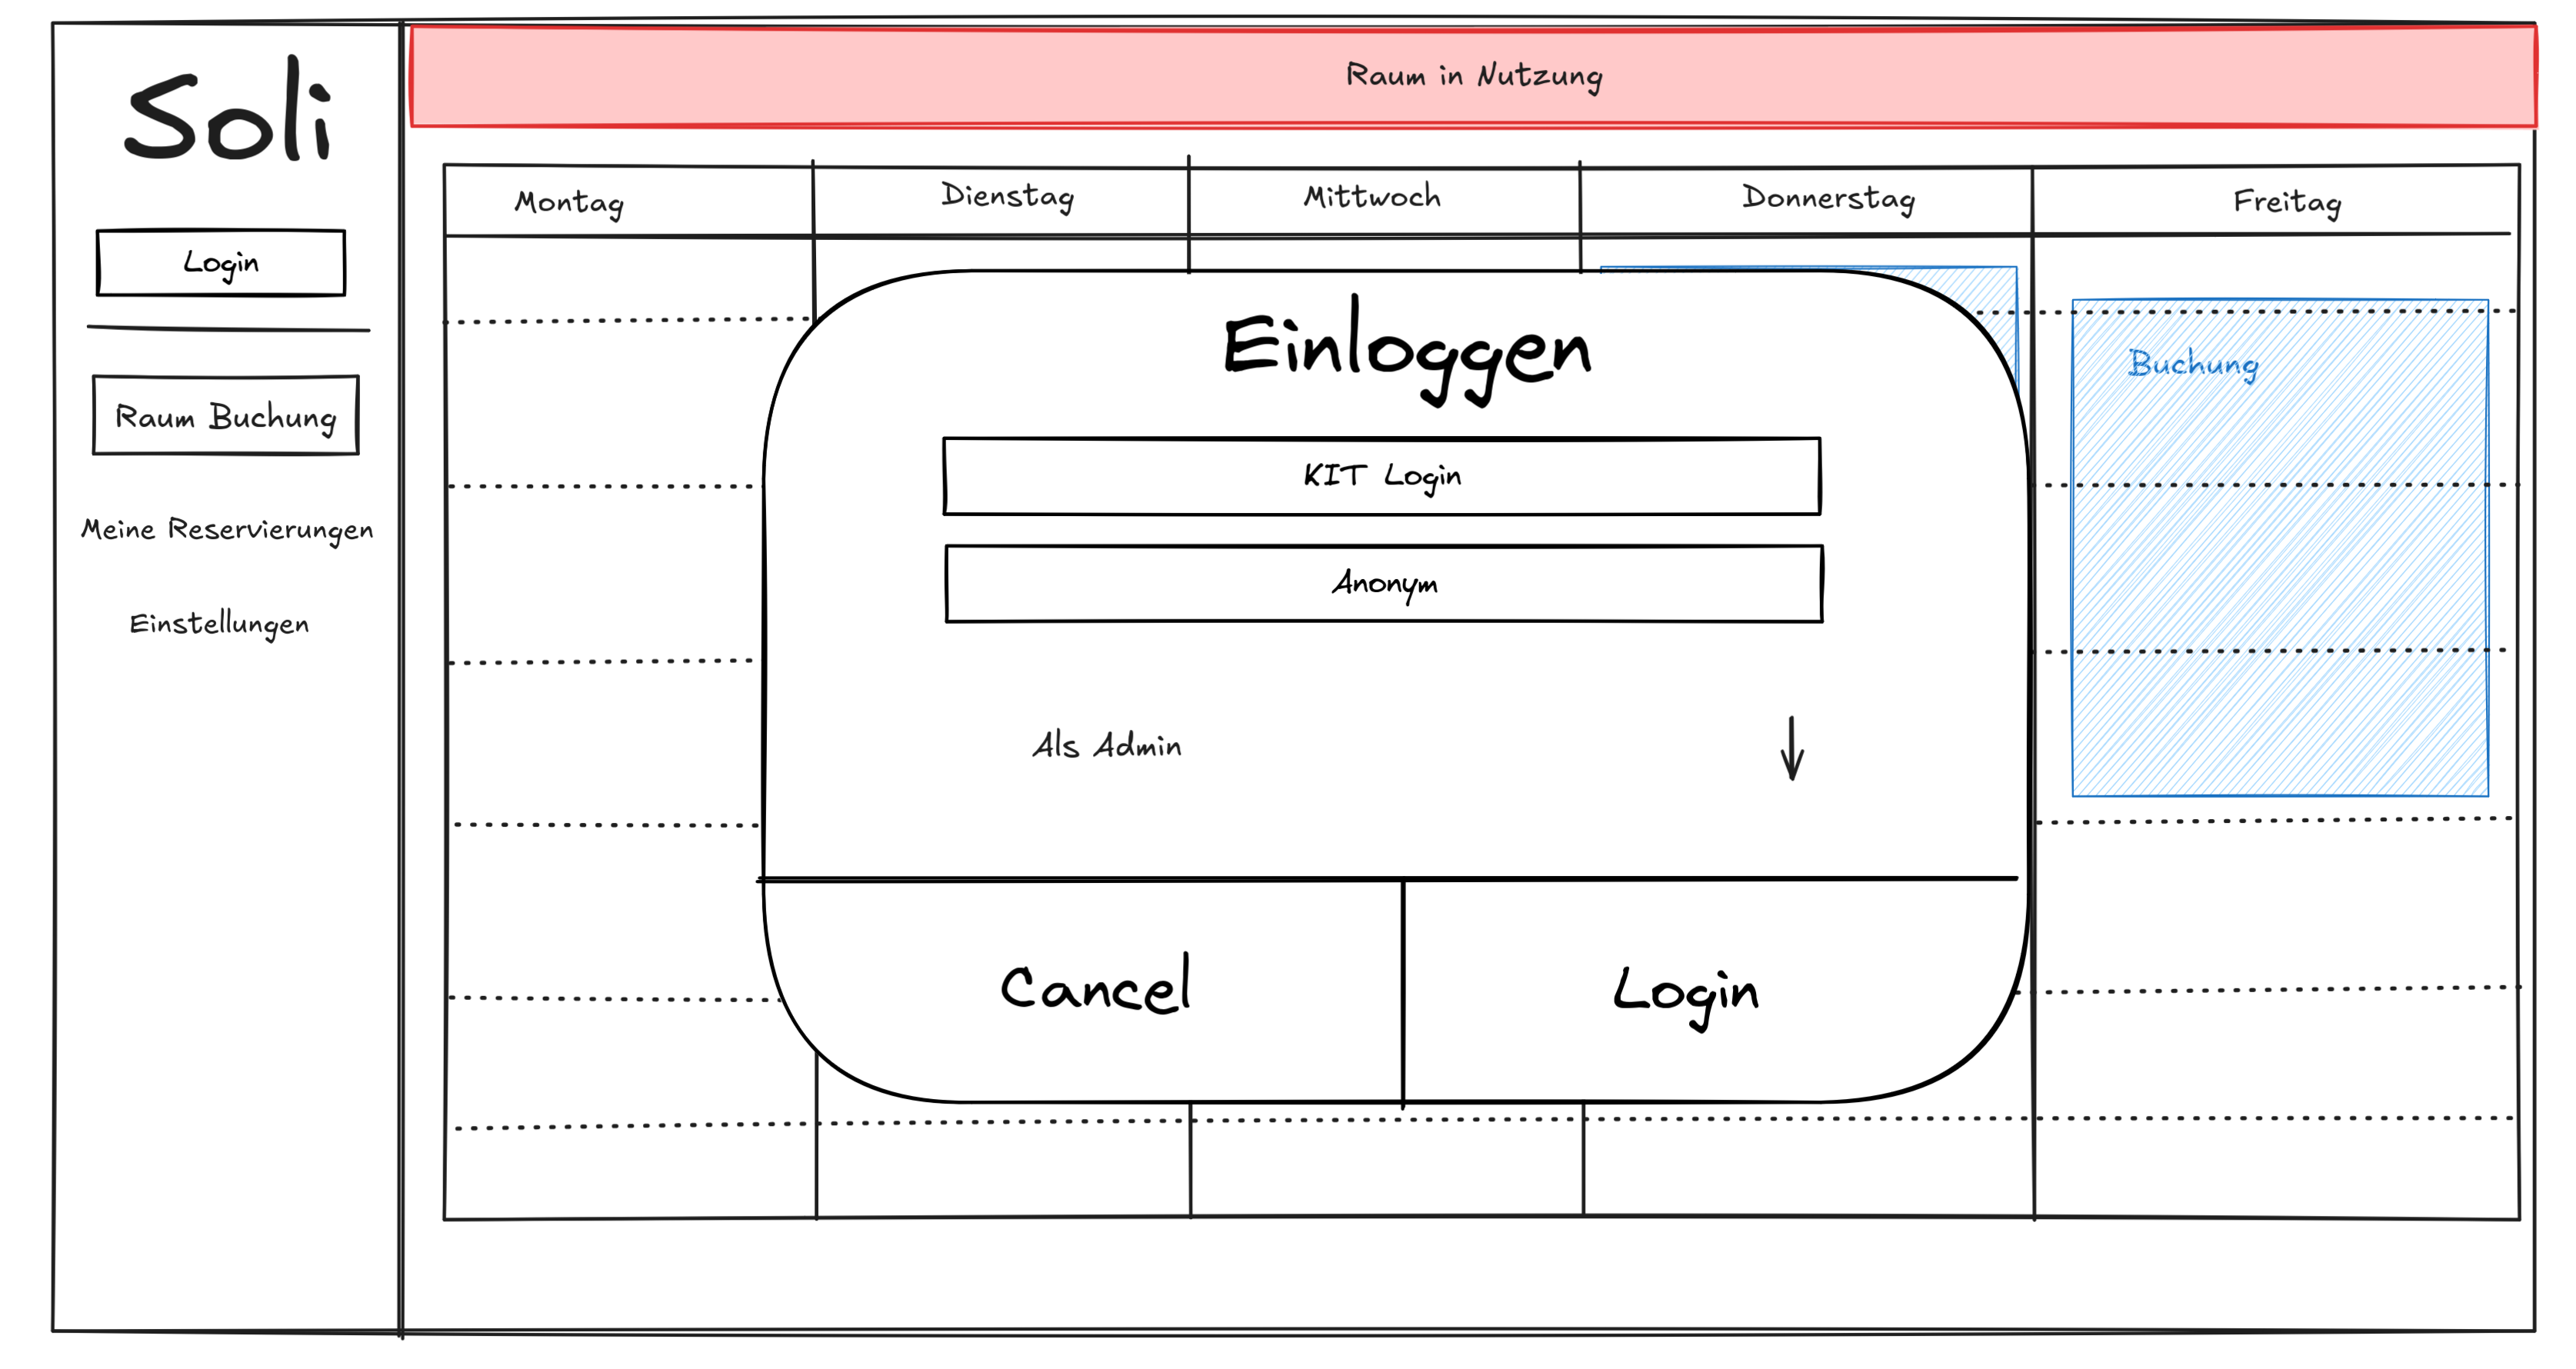
\includegraphics[scale=0.15]{figures/ui/anmeldungsseite}
    \caption{Anmeldungsseite}
    \label{fig:login}
\end{figure}
\clearpage

Sind Nutzende eingeloggt und belegen den Raum,
so wird ihnen die in Abbildung \ref{fig:checkout} dargestellte Ansicht angezeigt.
Hier können NutzerInnen den Raum wieder über den Quick-Checkout Button freigeben.
\begin{figure}[ht]
    \centering
    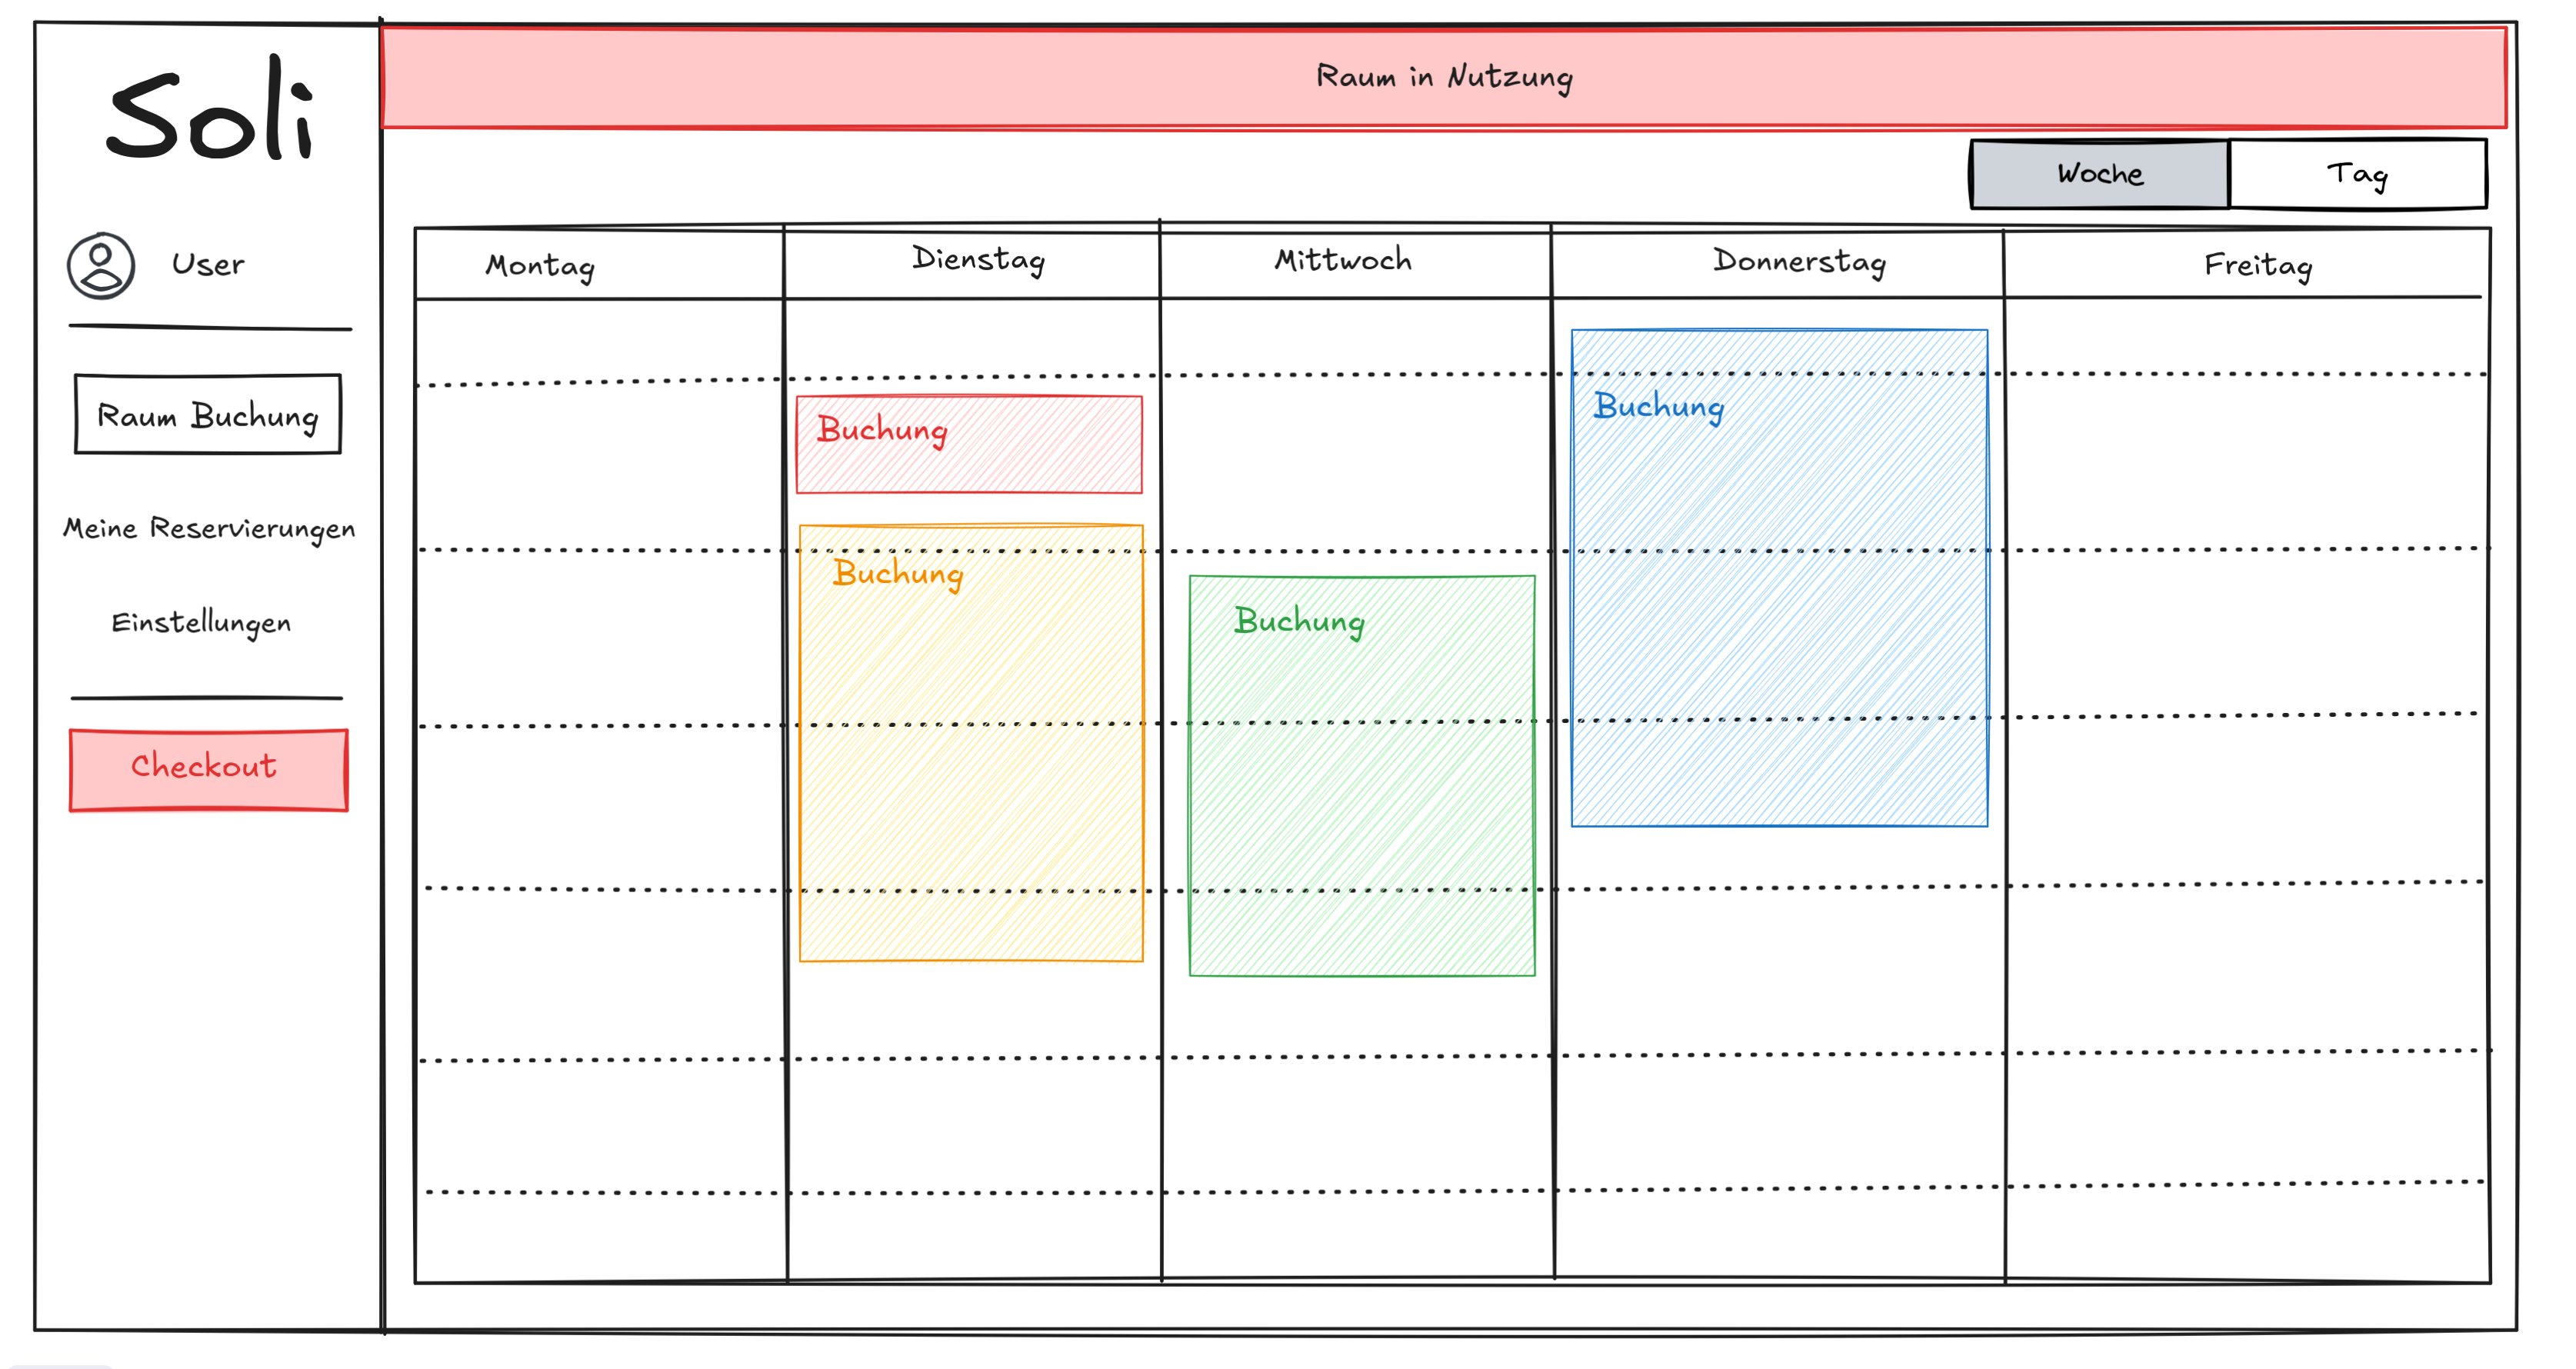
\includegraphics[scale=0.15]{figures/ui/checkout}
    \caption{Quick Checkout}
    \label{fig:checkout}
\end{figure}
\clearpage

\section{Buchungsverwaltung}
Sollte ein Benutzer eine Buchung vorgenommen haben, so kann dieser in der Reservierungsübersicht,
die in Abbildung \ref{fig:overview} dargestellt ist, seine Buchungen einsehen und verwalten.

\begin{figure}[ht]
    \includegraphics[scale=0.15]{figures/ui/reservierungsübersicht}
    \caption{Reservierungsübersicht}
    \label{fig:overview}
\end{figure}
\clearpage

\section{Adminstration}
Ein Administrator hat die Möglichkeit, über die Benutzeradminstrationsoberfläche,
die in Abbildung \ref{fig:adminuser} dargestellt ist, NutzerInnen einzusehen und zu verwalten.
So dient diese Ansicht z.B. dazu, Nutzende zu sperren oder zu entsperren.

\begin{figure}[ht]
    \centering
    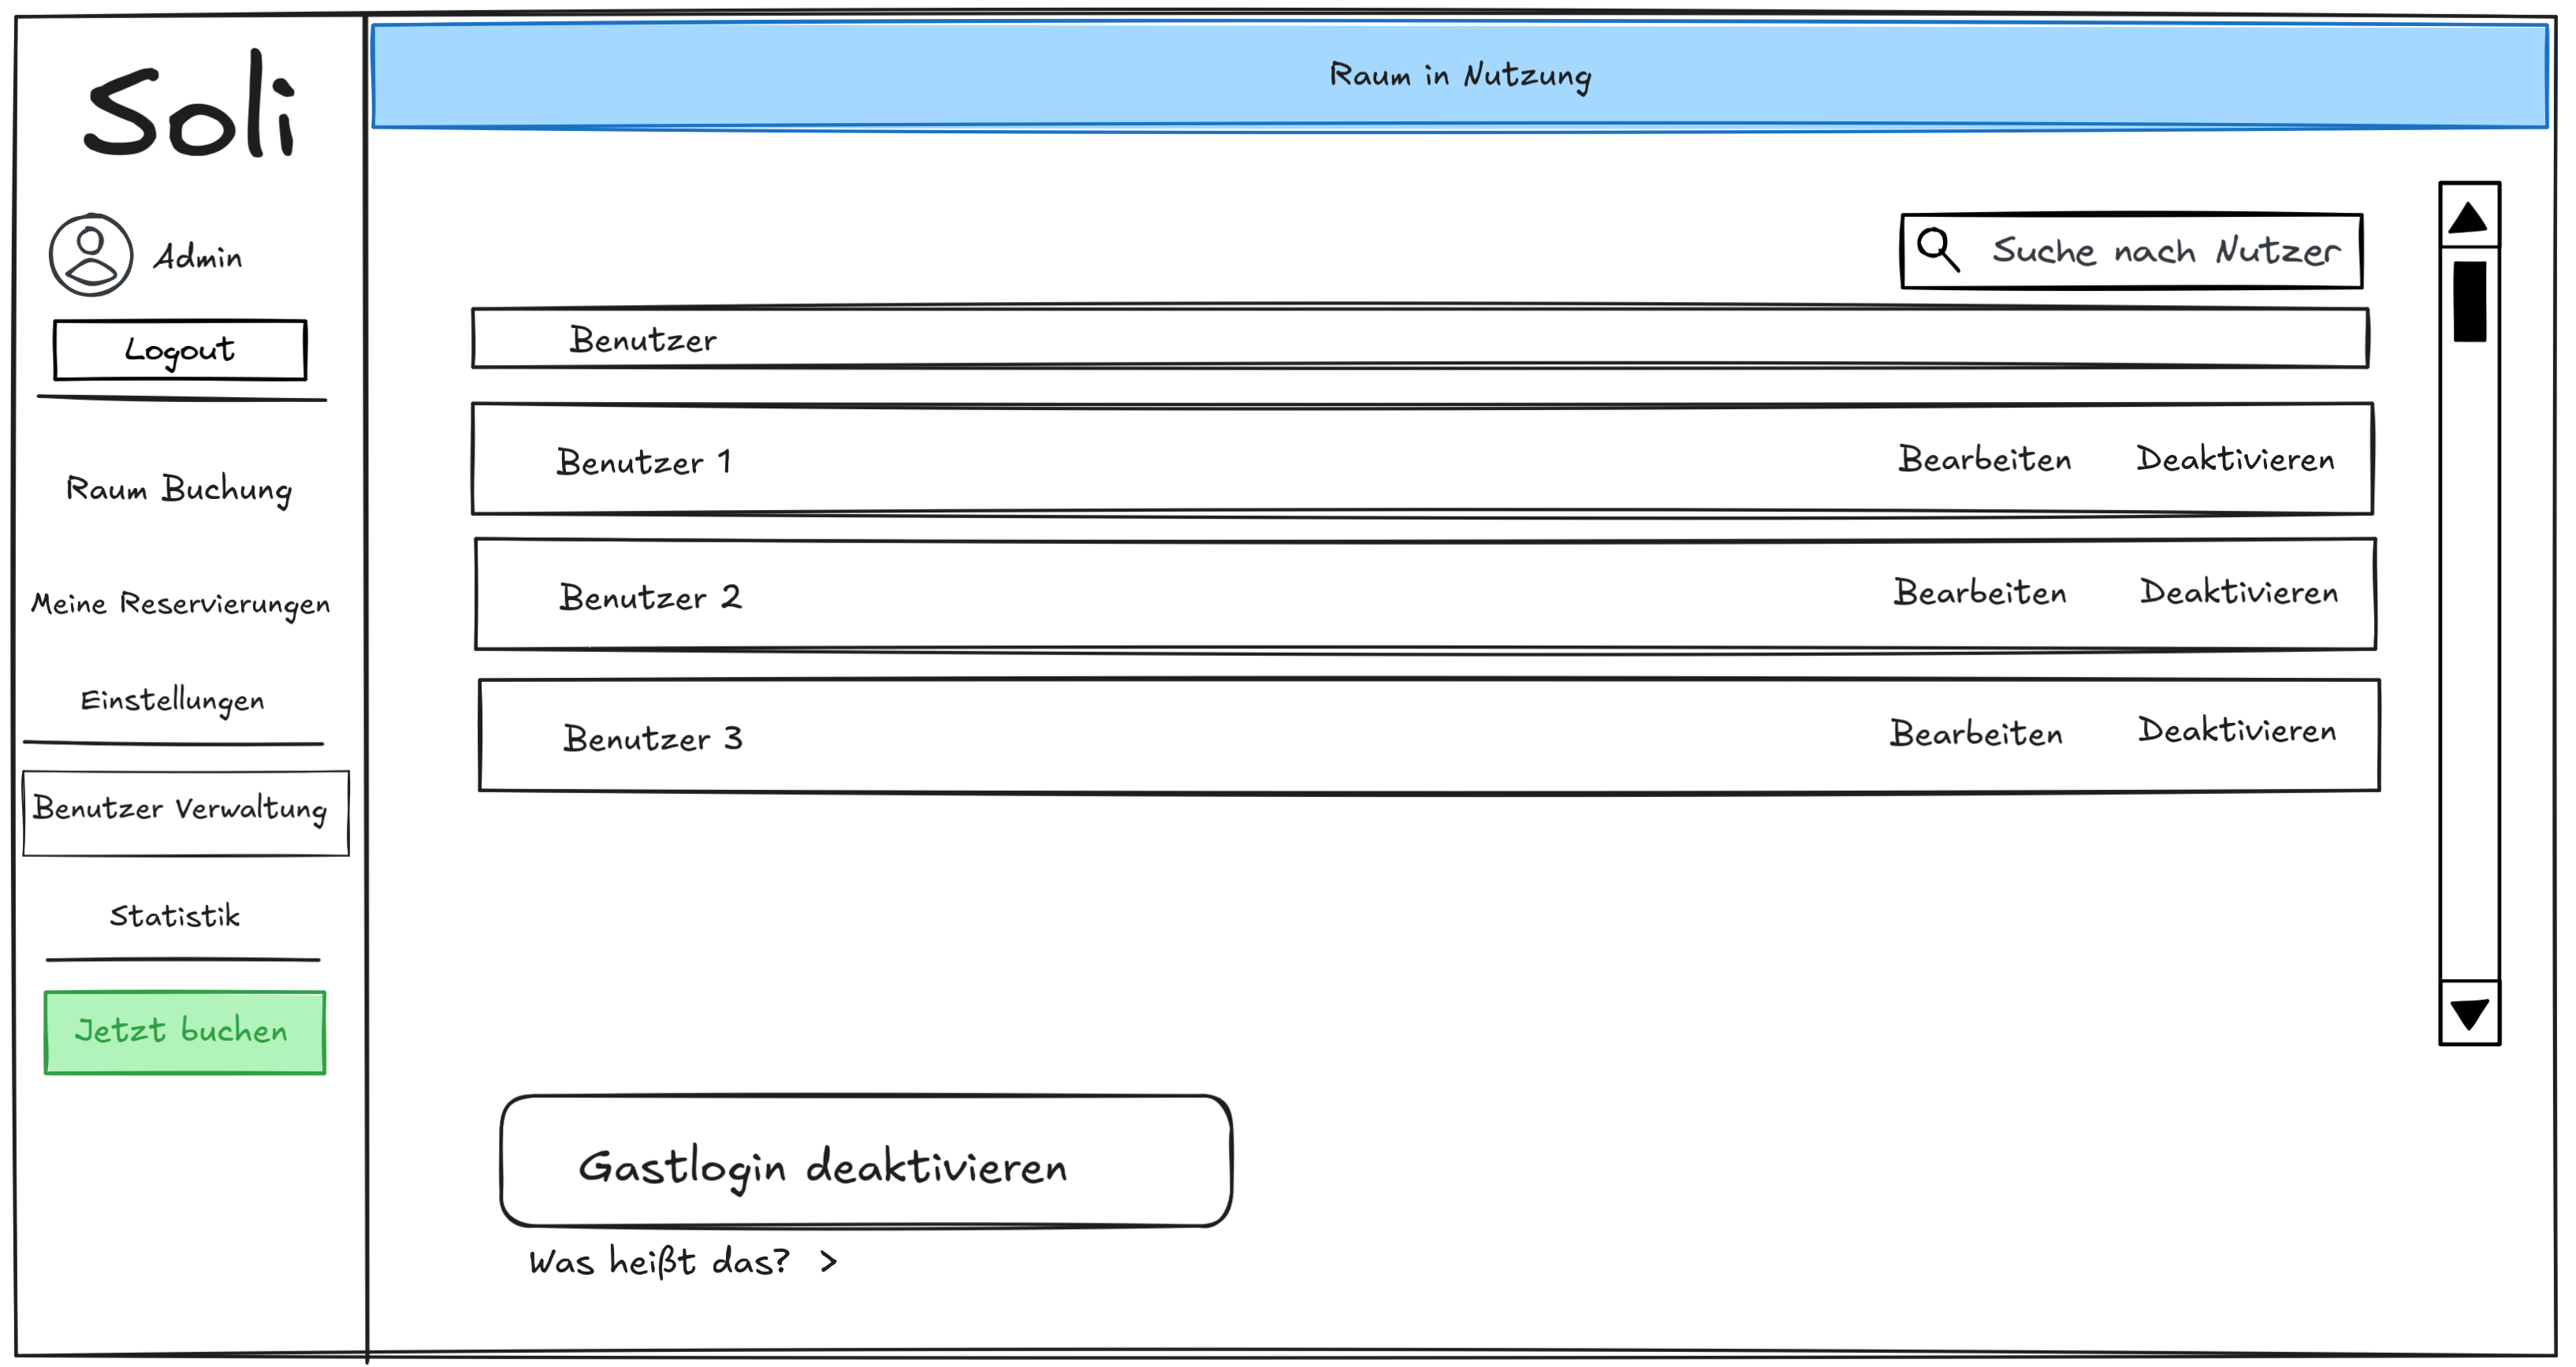
\includegraphics[scale=0.15]{figures/ui/useradminui}
    \caption{Benutzeradminstrationsoberfläche}
    \label{fig:adminuser}
\end{figure}

